	\chapter{Ergebnisse}
	\label{chap:ergebnisse}
	
	
	\section{Laufzeitskalierung bei mehreren Kernen}
	\label{sec:ergebnisparallel}
	Zuerst wird sichergestellt, dass sich die Observablen sowohl bei paralleler als auch bei serieller Modellierung gleich verhalten. Wie man an Bild~\ref{fig:vergleichham} sieht, ist das der Fall, die Ergebnisse des Hamiltonians liegen aufeinander und sind insbesondere in ihren Fehlergrenzen gleich. Dies gilt sowohl für die Parallelisierung mit OpenMP als auch mit MPI.
	
	\begin{figure}[htbp]
		% GNUPLOT: LaTeX picture with Postscript
\begingroup
  \makeatletter
  \providecommand\color[2][]{%
    \GenericError{(gnuplot) \space\space\space\@spaces}{%
      Package color not loaded in conjunction with
      terminal option `colourtext'%
    }{See the gnuplot documentation for explanation.%
    }{Either use 'blacktext' in gnuplot or load the package
      color.sty in LaTeX.}%
    \renewcommand\color[2][]{}%
  }%
  \providecommand\includegraphics[2][]{%
    \GenericError{(gnuplot) \space\space\space\@spaces}{%
      Package graphicx or graphics not loaded%
    }{See the gnuplot documentation for explanation.%
    }{The gnuplot epslatex terminal needs graphicx.sty or graphics.sty.}%
    \renewcommand\includegraphics[2][]{}%
  }%
  \providecommand\rotatebox[2]{#2}%
  \@ifundefined{ifGPcolor}{%
    \newif\ifGPcolor
    \GPcolortrue
  }{}%
  \@ifundefined{ifGPblacktext}{%
    \newif\ifGPblacktext
    \GPblacktextfalse
  }{}%
  % define a \g@addto@macro without @ in the name:
  \let\gplgaddtomacro\g@addto@macro
  % define empty templates for all commands taking text:
  \gdef\gplbacktext{}%
  \gdef\gplfronttext{}%
  \makeatother
  \ifGPblacktext
    % no textcolor at all
    \def\colorrgb#1{}%
    \def\colorgray#1{}%
  \else
    % gray or color?
    \ifGPcolor
      \def\colorrgb#1{\color[rgb]{#1}}%
      \def\colorgray#1{\color[gray]{#1}}%
      \expandafter\def\csname LTw\endcsname{\color{white}}%
      \expandafter\def\csname LTb\endcsname{\color{black}}%
      \expandafter\def\csname LTa\endcsname{\color{black}}%
      \expandafter\def\csname LT0\endcsname{\color[rgb]{1,0,0}}%
      \expandafter\def\csname LT1\endcsname{\color[rgb]{0,1,0}}%
      \expandafter\def\csname LT2\endcsname{\color[rgb]{0,0,1}}%
      \expandafter\def\csname LT3\endcsname{\color[rgb]{1,0,1}}%
      \expandafter\def\csname LT4\endcsname{\color[rgb]{0,1,1}}%
      \expandafter\def\csname LT5\endcsname{\color[rgb]{1,1,0}}%
      \expandafter\def\csname LT6\endcsname{\color[rgb]{0,0,0}}%
      \expandafter\def\csname LT7\endcsname{\color[rgb]{1,0.3,0}}%
      \expandafter\def\csname LT8\endcsname{\color[rgb]{0.5,0.5,0.5}}%
    \else
      % gray
      \def\colorrgb#1{\color{black}}%
      \def\colorgray#1{\color[gray]{#1}}%
      \expandafter\def\csname LTw\endcsname{\color{white}}%
      \expandafter\def\csname LTb\endcsname{\color{black}}%
      \expandafter\def\csname LTa\endcsname{\color{black}}%
      \expandafter\def\csname LT0\endcsname{\color{black}}%
      \expandafter\def\csname LT1\endcsname{\color{black}}%
      \expandafter\def\csname LT2\endcsname{\color{black}}%
      \expandafter\def\csname LT3\endcsname{\color{black}}%
      \expandafter\def\csname LT4\endcsname{\color{black}}%
      \expandafter\def\csname LT5\endcsname{\color{black}}%
      \expandafter\def\csname LT6\endcsname{\color{black}}%
      \expandafter\def\csname LT7\endcsname{\color{black}}%
      \expandafter\def\csname LT8\endcsname{\color{black}}%
    \fi
  \fi
    \setlength{\unitlength}{0.0500bp}%
    \ifx\gptboxheight\undefined%
      \newlength{\gptboxheight}%
      \newlength{\gptboxwidth}%
      \newsavebox{\gptboxtext}%
    \fi%
    \setlength{\fboxrule}{0.5pt}%
    \setlength{\fboxsep}{1pt}%
\begin{picture}(8640.00,6480.00)%
    \gplgaddtomacro\gplbacktext{%
      \csname LTb\endcsname%
      \put(946,704){\makebox(0,0)[r]{\strut{}$-2.2$}}%
      \put(946,1316){\makebox(0,0)[r]{\strut{}$-2$}}%
      \put(946,1929){\makebox(0,0)[r]{\strut{}$-1.8$}}%
      \put(946,2541){\makebox(0,0)[r]{\strut{}$-1.6$}}%
      \put(946,3153){\makebox(0,0)[r]{\strut{}$-1.4$}}%
      \put(946,3766){\makebox(0,0)[r]{\strut{}$-1.2$}}%
      \put(946,4378){\makebox(0,0)[r]{\strut{}$-1$}}%
      \put(946,4990){\makebox(0,0)[r]{\strut{}$-0.8$}}%
      \put(946,5603){\makebox(0,0)[r]{\strut{}$-0.6$}}%
      \put(946,6215){\makebox(0,0)[r]{\strut{}$-0.4$}}%
      \put(1078,484){\makebox(0,0){\strut{}$0$}}%
      \put(2511,484){\makebox(0,0){\strut{}$1$}}%
      \put(3944,484){\makebox(0,0){\strut{}$2$}}%
      \put(5377,484){\makebox(0,0){\strut{}$3$}}%
      \put(6810,484){\makebox(0,0){\strut{}$4$}}%
      \put(8243,484){\makebox(0,0){\strut{}$5$}}%
    }%
    \gplgaddtomacro\gplfronttext{%
      \csname LTb\endcsname%
      \put(176,3459){\rotatebox{-270}{\makebox(0,0){\strut{}$H/\text{laenge}^2$}}}%
      \put(4660,154){\makebox(0,0){\strut{}Temperatur}}%
      \csname LTb\endcsname%
      \put(4642,6042){\makebox(0,0)[r]{\strut{}zeilenweise durchgehen}}%
      \csname LTb\endcsname%
      \put(4642,5822){\makebox(0,0)[r]{\strut{}Schachbrettmuster parallel}}%
    }%
    \gplbacktext
    \put(0,0){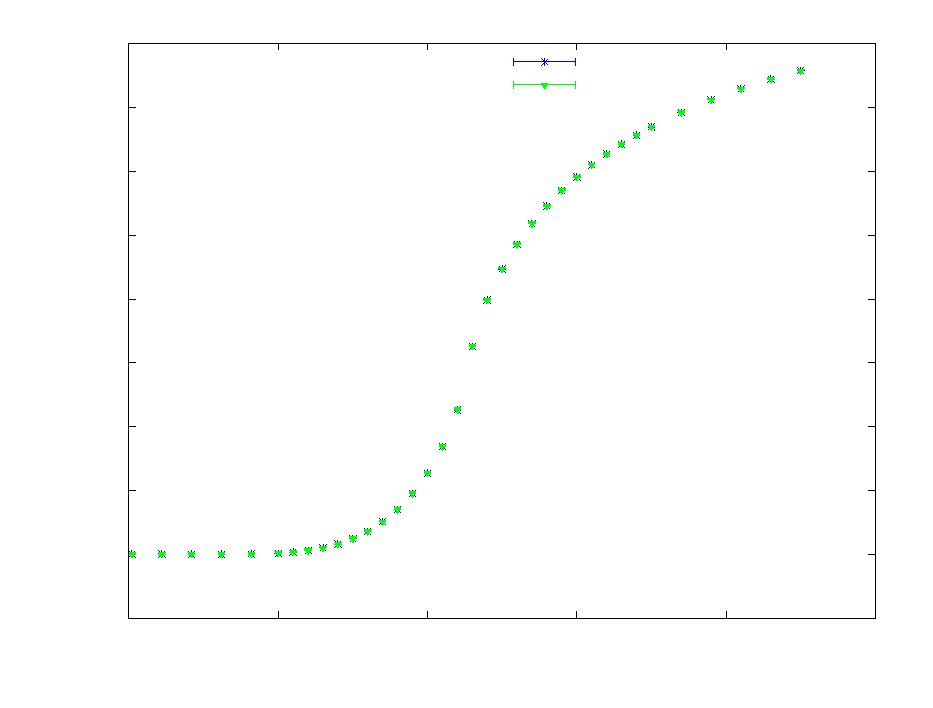
\includegraphics{vergleichham}}%
    \gplfronttext
  \end{picture}%
\endgroup

		\caption[Hamiltonian mit und ohne Parallelisierung]{Hamiltonian bei Gitterlänge 100 bei verschiedenen Temperaturen mit verschiedenen Parallelisierungsmethoden gemessen. Die Fehler sind mit Blocklänge 128 bestimmt und so klein, dass sie fast nicht sichtbar sind.}
		\label{fig:vergleichham}
	\end{figure}
	
	Die Graphiken in dieser Arbeit wurden mittels \texttt{gnuplot}\cite{gnuplotdoc}, im speziellen den Programmen \texttt{plot.gp} und \texttt{multiplot.gp} erstellt.
	
	\subsection{Skalierung mit OpenMP}
	\label{subsec:ergebnisseopenmp}
	
	Um zu ermitteln, mit wie vielen \textit{Threads} idealerweise gemessen werden sollte, wurde die Skalierung der \texttt{messenmehreregeneratoren}-Funktion betrachtet. Die Messungen werden wie in Abschnitt~\ref{subsec:paropenmp} beschrieben durchgeführt, dargestellt wird der Kehrwert des gemessenen Mittelwertes. Die Fehler werden wiederum mit Gaußscher Fehlerfortpflanzung bestimmt, aufgetragen ist somit der \textit{Speedup} nach der Definition aus Gl.~\ref{eq:speedup}.%Hierbei wurde für verschiedene Gitterlängen und Temperaturen die Zeit, die für 1.000 Ausführungen der sweep-Funktion benötigt wurde, gemessen. Von zehn solchen Messungen wurden mittels der Standardschätzer Mittelwert und Varianz gebildet. 
	
	\begin{figure}[htbp]
		\input{Bilder/speeduplaenge}
		\caption[\textit{Speedup} bei verschiedenen Gitterlängen bei Verwendung von OpenMP]{\textit{Speedup}  bei verschiedenen Gitterlängen bei Verwendung von OpenMP, Mittelwert über $10 \cdot 1000$ Messungen, gemessen bei $T=\num{0,5}$}
		\label{fig:skalierunglaenge}
	\end{figure}
	
	In Abbildung~\ref{fig:skalierunglaenge} ist die Skalierung bei verschiedenen Gitterlängen aufgetragen. Gemessen wurde auf der lcpunode02 des Clusterrechners QBiG. Hierbei handelt es sich um eine Intel(R) Xeon(R) CPU E5-2620 0 @2.00 GHz mit 12 Kernen.%(weitere Werte?).
	
	Bei kleinen Gitterlängen wie $L=10$ wird die Durchführung durch das Verwenden mehrerer \textit{Threads} nicht beschleunigt, der \textit{Overhead} der Parallelisierung verlangsamt die Durchführung sogar noch. Der minimale \textit{Speedup} ist hier $\num{0,56\pm0,01}$ bei 12 \textit{Threads}. Bei etwas größeren Gitterlängen wie z.{}B.{} $L=40$, wird die Funktion mit steigender Anzahl an \textit{Threads} erst schneller durchgeführt, ab einer gewissen Zahl an \textit{Threads}, hier $8$, überwiegt allerdings der \textit{Overhead} gegenüber der Beschleunigung durch mehr \textit{Threads} und der \textit{Speedup} wird mit steigender Anzahl der \textit{Threads} wieder kleiner. Die Fehler sind hier recht groß, da das Programm nicht lange für die Ausführung benötigt, nur ca.{} $\num{0,03}\si{\second}$ bei $7$ \textit{Threads}, sodass hier die natürlichen Variationen der Prozessoren aufgrund von Hitze o.{}Ä.{} zu einem großen relativen Fehler führen. Der maximale \textit{Speedup} ist $\num{3,57\pm0,45}$ bei sieben \textit{Threads}. Mit steigender Gitterlänge, hier im Beispiel $L=110$, wird der \textit{Overhead} im Vergleich zur Rechenzeit geringer, sodass der \textit{Speedup} mit der Anzahl der \textit{Threads} annähernd monoton ansteigt, und bei $12$ ein Maximum von $\num{5,26\pm0,14}$ hat.
	Bei größeren Gitterlängen wird der Einfluss des \textit{Overheads} nochmal geringer, wodurch der Anstieg des \textit{Speedups} steiler wird und bei Gitterlänge $L=500$ der maximale \textit{Speedup}, bei $12$ \textit{Threads}, $\num{5,99\pm0,12}$ beträgt. Jedoch ist dies auch das Maximum an Verbesserung, was mit OpenMP erreicht werden kann, die Werte der Gitterlänge $L=1260$ liegen in ihren Fehlergrenzen immer innerhalb der Fehler der Werte mit $L=500$.
 	
	%Wie man an Bild sieht, ist die Parallelisierung für kleine Gitterlängen sinnlos, es wird nur mehr overhead eingeführt und die benötigte Zeit steigt mit Anzahl der Cores.
	
	%Ab einer gewissen Gitterlänge sinkt die benötigte Rechenzeit mit mehr Cores, sinkt allerdings für mehr Cores, wenn es mehr Overhead gibt. Bei steigender Gitterlänge wird allerdings auch die Laufzeitverbesserung für mehr Cores sichtbar, es bildet sich erst ein Plateau, was für lange Gitterlängen schließlich in eine monoton steigende Funktion übergeht.
	
	Bei Gitterlängen ab $L=110$ entspricht das Verhalten des \textit{Speedups} somit den Erwartungen aus Abschnitt~\ref{sec:partheorie}. Daher werden ab einer Gitterlänge von $L=110$ die Messungen mit der maximalen Anzahl an \textit{Threads} durchgeführt, bei kleineren Gitterlängen wird auch eine entsprechend kleinere Anzahl an \textit{Threads} verwendet. 
	
	\subsection{Skalierung mit MPI}
	\label{subsec:ergebnissempi}
	
	Zum Untersuchen des Verhaltens bei Parallelisierung mit MPI wird die Ausführungsdauer der Funktion \texttt{messenmpi} bei verschiedenen Prozesszahlen wie in Abschnitt~\ref{subsec:parmpi} untersucht, die Ergebnisse für verschiedene Gitterlängen sind in Abb. \ref{fig:skalierunglaengempi} dargestellt. Die Messungen wurden auf den Nodes lnode[02-11] von QBiG durchgeführt.
	
		\begin{figure}[htbp]
			\input{Bilder/speeduplaengempi}
			\caption[\textit{Speedup} bei verschiedenen Gitterlängen bei Verwendung von MPI]{\textit{Speedup} bei verschiedenen Gitterlängen bei Verwendung von MPI, Mittelwert über $10 \cdot 1000$ Messungen, gemessen bei $T=\num{0,5}$}
			\label{fig:skalierunglaengempi}
		\end{figure}
		
	Prinzipiell ist das Verhalten ähnlich wie bei der Skalierung mit OpenMP: Bei niedrigen Gitterlängen wie $L=12$ dauert das Programm mit mehr Prozessen länger, hier ist der minimale \textit{Speedup} $\num{0,66\pm0,11}$ bei sechs MPI-Prozessen. Bei etwas längeren Gittern wie bei $L=60$ kommt es bei mehr Prozessen erst zu einer Verkürzung der Laufzeit, ab einem gewissen Punkt, hier \textit{Speedup} $\num{4,16\pm0,67}$ bei zehn Prozessen, jedoch wieder zu einer Verlangsamung. Bei noch größeren Gitterlängen wie $L=240$ bildet sich ein Plateau bei großen Prozesszahlen, hier mit \textit{Speedup} $\num{9,98\pm 0,67}$ bei 16 Prozessen. Mit steigender Gitterlänge liegen die Messwerte immer näher an der Gerade \enquote{\textit{Speedup}=Prozesszahl}, bei $L=840$ ist der maximale \textit{Speedup} $\num{16,93\pm0,24}$ bei 20 Prozessen, bei $L=1260$ $\num{17,24\pm0,11}$. Auch hier wird der Zuwachs der Verbesserung bei steigender Gitterlänge immer kleiner, die Werte für $L=840$ und $L=1260$ liegen fast aufeinander. Es ist nicht bei jeder Prozessanzahl ein Messwert vorhanden, da die Gitterlänge ein Vielfaches der verwendeten Prozesse sein muss.
	Auch hier entspricht das Verhalten den Erwartungen aus Absatz~\ref{sec:partheorie}, allerdings erst ab Gitterlänge $L=240$.

\subsection{Vergleich der Parallelisierungsmethoden}
%	
	\begin{figure}[htbp]
		\input{Bilder/speeduptemperaturmultiplot}
		\caption[\textit{Speedup}  bei verschiedenen Temperaturen]{\textit{Speedup} bei verschiedenen Temperaturen, Mittelwert über $10 \cdot 1000$ Messungen, gemessen bei Gitterlänge 500 bei OpenMP und 480 bei MPI}
		\label{fig:skalierungtemp}
	\end{figure}
	
	%Vergleich nicht gut, da Gitter nicht thermalisiert
	In Abb.~\ref{fig:skalierungtemp} ist die Laufzeitskalierung der beiden Parallelisierungsmethoden gegenübergestellt. 
	%In beiden Fällen wurde eine Gitterlänge gewählt, bei der der \textit{Speedup} in der Nähe des Maximums ist, und bei verschiedenen Temperaturen vergleichen. Für niedrigere Temperaturen ist der \textit{Speedup} minimal kleiner, die Messwerte liegen um ca.{} eine Standarabweichung auseinander. Im Fall von OpenMP ist der Unterschied $\num{0,17}$, im Fall von MPI $\num{0,50}$. In beide Graphiken ist zusätzlich die Gerade \enquote{\textit{Speedup}=Prozesszahl} eingezeichnet.
	In beiden Fällen wurde eine Gitterlänge gewählt, bei der der \textit{Speedup} in der Nähe des Maximums ist, und bei verschiedenen Temperaturen vergleichen. Für niedrigere Temperaturen ist der \textit{Speedup} kleiner, im Fall von OpenMP ist der Unterschied $\num{0,77}$, im Fall von MPI $\num{0,59}$. Bei den Messungen mit MPI liegen die \textit{Speedups} jedoch innerhalb der Fehlergrenzen der anderen \textit{Speedups}, der relative Unterschied ist kleiner.
	In beide Graphiken ist zusätzlich die Gerade \enquote{\textit{Speedup}=Prozesszahl} eingezeichnet.
	Beim Vergleich der Graphiken wird deutlich, dass mit MPI ein größerer \textit{Speedup} pro zusätzlichem Kern erreicht werden kann, bei 12 Threads bzw. Prozessen ist der Speedup des MPI-Programms bei Temperatur $T=\num{0,5}$ $\num{1,85}$-mal so groß wie bei OpenMP. Zudem ist bei MPI der Anstieg des Speedups gleichmäßiger als bei OpenMP. Bei Verwendung von MPI ist jedoch die mögliche Zahl an Prozessen bzw.{} die erlaubten Gitterlängen für eine feste Prozesszahl eingeschränkt, da die Gitterlänge durch die Prozesszahl teilbar und gerade sein muss, was bei OpenMP weniger der Fall ist, dort muss die Gitterlänge nur gerade sein.. Außerdem ist für die Benutzung von MPI eine Restrukturierung des gesamten Programms notwendig und es ist schwieriger, mit In/Output des Programms umzugehen. Beide Parallelisierungsmethoden führen jedoch zu den in Absatz~\ref{sec:partheorie} erwarteten Laufzeitverbesserungen.
	%OpenMP: 8 zusätzlihe zeilen in sweepfunktion, MPI: eingezeichnet.%allerdings liegen alle Messwerte in den Fehlergrenzen der adneren Messwerte bei gleicher Thread- bzw.{} Prozessanzahl.
	%gitterlänge an Maximum, temperatur? Unterschiede, aber innerhalb der fehlergrenzen
%	Zusätzlich gerade in Diagramm, MPI näher an gerade dran, besserer Verlauf. aber: beide entsprechen erwartungen, OpenMP mit viel weniger Zeilen und auch auf privatem  Rechner umsetzbar.
%		
%	Wenn man die Skalierung bei verschiedenen Temperaturen betrachtet, siehe Abb.~\ref{fig:skalierungtemp}, gibt es auch hier Unterschiede bei konstanter Gitterlänge: für niedrigere Temperaturen ist die Laufzeit geringer, allerdings der maximale \textit{Speedup} kleiner. Vermutlich kommt dies daher, dass bei niedrigen Temperaturen die Akzeptanzrate geringer ist und somit seltener eine Addition beim Hamiltonian durchgeführt werden muss. Diese Unterschiede entsprechen ungefähr einer Standardabweichung, dies ist allerdings recht gering und selbst beim größten \textit{Speedup} beträgt der Unterschied wischen den Temperaturen nur $\num{0,17}$.
	%Bild Werte übereinander->gleich Auch Hamiltonian als Vergleich? Magnetisierung passt, aber Werte von QBiG abwarten.
	%Skalierung auf QBiG?
	
	%Da im Folgenden das Verhalten bei großen Gitterlängen betrachtet wird, wird nach Möglichkeit mit der maximalen Anzahl an Kernen gerechnet. 
	%Insgesamt entspricht somit die Skalierung bei hohen Gitterlängen dem Ahmdahlschen Gesetz.
	%Messungen der Parallelisierung von messen/sweep auf lcpunode02 in QBiG: Bis zu 12 Kerne. Kennwerte von lcpunode02?

	%Parallelisierung Bootstrap?
	
	%Zuerst: Vergleich der verschiedenen sweep-Funktionen: Hamiltonian gleich. Bild.
	
	%Skalierung auf lcpunode2: Vergleich zwei Schleifen/tryflip/Temperaturen?
	%Bild von idealem Code, Skalierung wie erwartet (nach Ahmdahls law?)
	
	\section{Verhalten der beobachteten Observablen}
	\label{sec:ergebnisobservablen}
	
	Die folgenden Ergebnisse wurden alle mit Verwendung von OpenMP bestimmt.
	In Bild~\ref{fig:ergebnisakzeptanzrate} ist die Akzeptanzrate als Funktion von der Temperatur dargestellt. Bei kleinen Temperaturen ist sie null, steigt ab ca. $T=1$ an, hat bei ca. $T=\num{2,3}$ einen Wendepunkt mit Akzeptanzrate ca. $\num{0,2}$ und nähert sich danach asymptotisch dem Wert $1$. 
	
	%Die Varianz der Akzeptanzrate ist bei geringer Temperatur sehr klein, ca.{} $10^{-8}$ , wird im Bereich um $T=\num{2,2}$ groß, mit Maximalwert ca.{} $10^{-3}}$, und danach wieder kleiner, ca.{} $10^{-4}$.
	
	\begin{figure}[htbp]
		% GNUPLOT: LaTeX picture with Postscript
\begingroup
  \makeatletter
  \providecommand\color[2][]{%
    \GenericError{(gnuplot) \space\space\space\@spaces}{%
      Package color not loaded in conjunction with
      terminal option `colourtext'%
    }{See the gnuplot documentation for explanation.%
    }{Either use 'blacktext' in gnuplot or load the package
      color.sty in LaTeX.}%
    \renewcommand\color[2][]{}%
  }%
  \providecommand\includegraphics[2][]{%
    \GenericError{(gnuplot) \space\space\space\@spaces}{%
      Package graphicx or graphics not loaded%
    }{See the gnuplot documentation for explanation.%
    }{The gnuplot epslatex terminal needs graphicx.sty or graphics.sty.}%
    \renewcommand\includegraphics[2][]{}%
  }%
  \providecommand\rotatebox[2]{#2}%
  \@ifundefined{ifGPcolor}{%
    \newif\ifGPcolor
    \GPcolortrue
  }{}%
  \@ifundefined{ifGPblacktext}{%
    \newif\ifGPblacktext
    \GPblacktextfalse
  }{}%
  % define a \g@addto@macro without @ in the name:
  \let\gplgaddtomacro\g@addto@macro
  % define empty templates for all commands taking text:
  \gdef\gplbacktext{}%
  \gdef\gplfronttext{}%
  \makeatother
  \ifGPblacktext
    % no textcolor at all
    \def\colorrgb#1{}%
    \def\colorgray#1{}%
  \else
    % gray or color?
    \ifGPcolor
      \def\colorrgb#1{\color[rgb]{#1}}%
      \def\colorgray#1{\color[gray]{#1}}%
      \expandafter\def\csname LTw\endcsname{\color{white}}%
      \expandafter\def\csname LTb\endcsname{\color{black}}%
      \expandafter\def\csname LTa\endcsname{\color{black}}%
      \expandafter\def\csname LT0\endcsname{\color[rgb]{1,0,0}}%
      \expandafter\def\csname LT1\endcsname{\color[rgb]{0,1,0}}%
      \expandafter\def\csname LT2\endcsname{\color[rgb]{0,0,1}}%
      \expandafter\def\csname LT3\endcsname{\color[rgb]{1,0,1}}%
      \expandafter\def\csname LT4\endcsname{\color[rgb]{0,1,1}}%
      \expandafter\def\csname LT5\endcsname{\color[rgb]{1,1,0}}%
      \expandafter\def\csname LT6\endcsname{\color[rgb]{0,0,0}}%
      \expandafter\def\csname LT7\endcsname{\color[rgb]{1,0.3,0}}%
      \expandafter\def\csname LT8\endcsname{\color[rgb]{0.5,0.5,0.5}}%
    \else
      % gray
      \def\colorrgb#1{\color{black}}%
      \def\colorgray#1{\color[gray]{#1}}%
      \expandafter\def\csname LTw\endcsname{\color{white}}%
      \expandafter\def\csname LTb\endcsname{\color{black}}%
      \expandafter\def\csname LTa\endcsname{\color{black}}%
      \expandafter\def\csname LT0\endcsname{\color{black}}%
      \expandafter\def\csname LT1\endcsname{\color{black}}%
      \expandafter\def\csname LT2\endcsname{\color{black}}%
      \expandafter\def\csname LT3\endcsname{\color{black}}%
      \expandafter\def\csname LT4\endcsname{\color{black}}%
      \expandafter\def\csname LT5\endcsname{\color{black}}%
      \expandafter\def\csname LT6\endcsname{\color{black}}%
      \expandafter\def\csname LT7\endcsname{\color{black}}%
      \expandafter\def\csname LT8\endcsname{\color{black}}%
    \fi
  \fi
    \setlength{\unitlength}{0.0500bp}%
    \ifx\gptboxheight\undefined%
      \newlength{\gptboxheight}%
      \newlength{\gptboxwidth}%
      \newsavebox{\gptboxtext}%
    \fi%
    \setlength{\fboxrule}{0.5pt}%
    \setlength{\fboxsep}{1pt}%
\begin{picture}(8640.00,4320.00)%
    \gplgaddtomacro\gplbacktext{%
      \csname LTb\endcsname%
      \put(1164,737){\makebox(0,0)[r]{\strut{}$0$}}%
      \put(1164,1394){\makebox(0,0)[r]{\strut{}$0.2$}}%
      \put(1164,2051){\makebox(0,0)[r]{\strut{}$0.4$}}%
      \put(1164,2708){\makebox(0,0)[r]{\strut{}$0.6$}}%
      \put(1164,3365){\makebox(0,0)[r]{\strut{}$0.8$}}%
      \put(1164,4022){\makebox(0,0)[r]{\strut{}$1$}}%
      \put(1299,484){\makebox(0,0){\strut{}$0$}}%
      \put(1990,484){\makebox(0,0){\strut{}$2000$}}%
      \put(2680,484){\makebox(0,0){\strut{}$4000$}}%
      \put(3370,484){\makebox(0,0){\strut{}$6000$}}%
      \put(4061,484){\makebox(0,0){\strut{}$8000$}}%
      \put(4751,484){\makebox(0,0){\strut{}$10000$}}%
    }%
    \gplgaddtomacro\gplfronttext{%
      \csname LTb\endcsname%
      \put(526,2379){\rotatebox{-270}{\makebox(0,0){\strut{}Akzeptanzrate}}}%
      \put(3023,154){\makebox(0,0){\strut{}Temperatur}}%
    }%
    \gplgaddtomacro\gplbacktext{%
      \csname LTb\endcsname%
      \put(4620,737){\makebox(0,0)[r]{\strut{}}}%
      \put(4620,1394){\makebox(0,0)[r]{\strut{}}}%
      \put(4620,2051){\makebox(0,0)[r]{\strut{}}}%
      \put(4620,2708){\makebox(0,0)[r]{\strut{}}}%
      \put(4620,3365){\makebox(0,0)[r]{\strut{}}}%
      \put(4620,4022){\makebox(0,0)[r]{\strut{}}}%
      \put(4752,484){\makebox(0,0){\strut{}$0$}}%
      \put(5443,484){\makebox(0,0){\strut{}$1$}}%
      \put(6134,484){\makebox(0,0){\strut{}$2$}}%
      \put(6825,484){\makebox(0,0){\strut{}$3$}}%
      \put(7516,484){\makebox(0,0){\strut{}$4$}}%
      \put(8207,484){\makebox(0,0){\strut{}$5$}}%
    }%
    \gplgaddtomacro\gplfronttext{%
      \csname LTb\endcsname%
      \put(6479,154){\makebox(0,0){\strut{}Temperatur}}%
    }%
    \gplbacktext
    \put(0,0){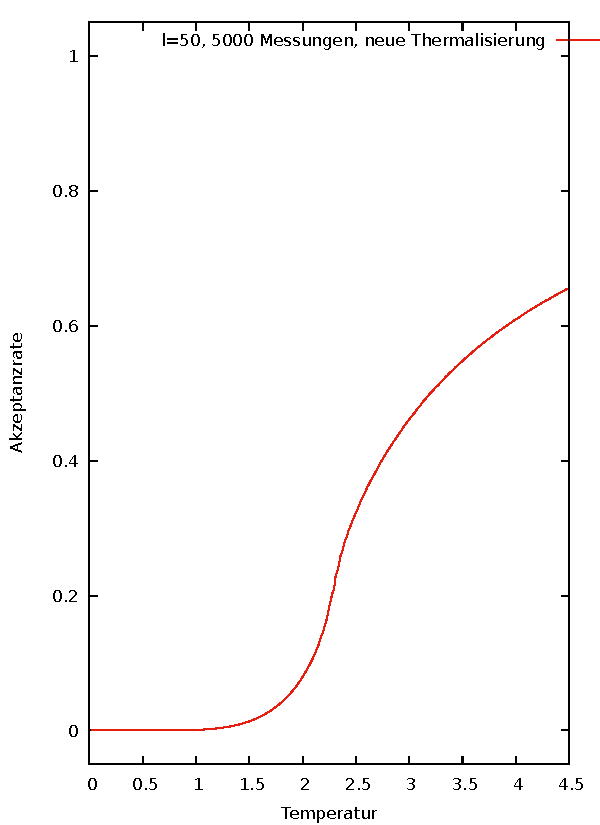
\includegraphics{akzeptanzrate}}%
    \gplfronttext
  \end{picture}%
\endgroup

		\caption[Akzeptanzrate in Abhängigkeit von der Temperatur]{Akzeptanzrate in Abhängigkeit von der Temperatur, gemessen bei Gitterlänge 100, mit Blocklänge 128 zur Fehlerberechnung. Die Fehler sind so klein, dass sie fast nicht sichtbar sind. Dargestellt ist sowohl die Umgebung des kritischen Punktes als auch das asymptotische Verhalten.}
		\label{fig:ergebnisakzeptanzrate}
	\end{figure}
	
	Der Hamiltonian verhält sich qualitativ ähnlich, siehe Bild~\ref{fig:ergebnishamiltonian}. Bei geringen Temperaturen hat er den Wert $-2\cdot\text{laenge}^2$, was auf ein vollkommen homogen ausgerichtetes Gitter hinweist. Bei ca.{} $T=\num{2,3}$ beträgt der Hamiltonian ca.{} $-\num{1,4}\cdot\text{laenge}^2$ und nähert sich dann asymptotisch null.
	
	%Auch hier ist die Varianz anfangs klein, ca.{} 
	
	
	
	\begin{figure}[htbp]
		% GNUPLOT: LaTeX picture with Postscript
\begingroup
  \makeatletter
  \providecommand\color[2][]{%
    \GenericError{(gnuplot) \space\space\space\@spaces}{%
      Package color not loaded in conjunction with
      terminal option `colourtext'%
    }{See the gnuplot documentation for explanation.%
    }{Either use 'blacktext' in gnuplot or load the package
      color.sty in LaTeX.}%
    \renewcommand\color[2][]{}%
  }%
  \providecommand\includegraphics[2][]{%
    \GenericError{(gnuplot) \space\space\space\@spaces}{%
      Package graphicx or graphics not loaded%
    }{See the gnuplot documentation for explanation.%
    }{The gnuplot epslatex terminal needs graphicx.sty or graphics.sty.}%
    \renewcommand\includegraphics[2][]{}%
  }%
  \providecommand\rotatebox[2]{#2}%
  \@ifundefined{ifGPcolor}{%
    \newif\ifGPcolor
    \GPcolortrue
  }{}%
  \@ifundefined{ifGPblacktext}{%
    \newif\ifGPblacktext
    \GPblacktextfalse
  }{}%
  % define a \g@addto@macro without @ in the name:
  \let\gplgaddtomacro\g@addto@macro
  % define empty templates for all commands taking text:
  \gdef\gplbacktext{}%
  \gdef\gplfronttext{}%
  \makeatother
  \ifGPblacktext
    % no textcolor at all
    \def\colorrgb#1{}%
    \def\colorgray#1{}%
  \else
    % gray or color?
    \ifGPcolor
      \def\colorrgb#1{\color[rgb]{#1}}%
      \def\colorgray#1{\color[gray]{#1}}%
      \expandafter\def\csname LTw\endcsname{\color{white}}%
      \expandafter\def\csname LTb\endcsname{\color{black}}%
      \expandafter\def\csname LTa\endcsname{\color{black}}%
      \expandafter\def\csname LT0\endcsname{\color[rgb]{1,0,0}}%
      \expandafter\def\csname LT1\endcsname{\color[rgb]{0,1,0}}%
      \expandafter\def\csname LT2\endcsname{\color[rgb]{0,0,1}}%
      \expandafter\def\csname LT3\endcsname{\color[rgb]{1,0,1}}%
      \expandafter\def\csname LT4\endcsname{\color[rgb]{0,1,1}}%
      \expandafter\def\csname LT5\endcsname{\color[rgb]{1,1,0}}%
      \expandafter\def\csname LT6\endcsname{\color[rgb]{0,0,0}}%
      \expandafter\def\csname LT7\endcsname{\color[rgb]{1,0.3,0}}%
      \expandafter\def\csname LT8\endcsname{\color[rgb]{0.5,0.5,0.5}}%
    \else
      % gray
      \def\colorrgb#1{\color{black}}%
      \def\colorgray#1{\color[gray]{#1}}%
      \expandafter\def\csname LTw\endcsname{\color{white}}%
      \expandafter\def\csname LTb\endcsname{\color{black}}%
      \expandafter\def\csname LTa\endcsname{\color{black}}%
      \expandafter\def\csname LT0\endcsname{\color{black}}%
      \expandafter\def\csname LT1\endcsname{\color{black}}%
      \expandafter\def\csname LT2\endcsname{\color{black}}%
      \expandafter\def\csname LT3\endcsname{\color{black}}%
      \expandafter\def\csname LT4\endcsname{\color{black}}%
      \expandafter\def\csname LT5\endcsname{\color{black}}%
      \expandafter\def\csname LT6\endcsname{\color{black}}%
      \expandafter\def\csname LT7\endcsname{\color{black}}%
      \expandafter\def\csname LT8\endcsname{\color{black}}%
    \fi
  \fi
    \setlength{\unitlength}{0.0500bp}%
    \ifx\gptboxheight\undefined%
      \newlength{\gptboxheight}%
      \newlength{\gptboxwidth}%
      \newsavebox{\gptboxtext}%
    \fi%
    \setlength{\fboxrule}{0.5pt}%
    \setlength{\fboxsep}{1pt}%
\begin{picture}(8640.00,4320.00)%
    \gplgaddtomacro\gplbacktext{%
      \csname LTb\endcsname%
      \put(1164,721){\makebox(0,0)[r]{\strut{}$-2$}}%
      \put(1164,1550){\makebox(0,0)[r]{\strut{}$-1.5$}}%
      \put(1164,2380){\makebox(0,0)[r]{\strut{}$-1$}}%
      \put(1164,3209){\makebox(0,0)[r]{\strut{}$-0.5$}}%
      \put(1164,4038){\makebox(0,0)[r]{\strut{}$0$}}%
      \put(1299,484){\makebox(0,0){\strut{}$0$}}%
      \put(1990,484){\makebox(0,0){\strut{}$2000$}}%
      \put(2680,484){\makebox(0,0){\strut{}$4000$}}%
      \put(3370,484){\makebox(0,0){\strut{}$6000$}}%
      \put(4061,484){\makebox(0,0){\strut{}$8000$}}%
      \put(4751,484){\makebox(0,0){\strut{}$10000$}}%
    }%
    \gplgaddtomacro\gplfronttext{%
      \csname LTb\endcsname%
      \put(394,2379){\rotatebox{-270}{\makebox(0,0){\strut{}$H/\text{laenge}^2$}}}%
      \put(3023,154){\makebox(0,0){\strut{}Temperatur}}%
    }%
    \gplgaddtomacro\gplbacktext{%
      \csname LTb\endcsname%
      \put(4620,721){\makebox(0,0)[r]{\strut{}}}%
      \put(4620,1550){\makebox(0,0)[r]{\strut{}}}%
      \put(4620,2380){\makebox(0,0)[r]{\strut{}}}%
      \put(4620,3209){\makebox(0,0)[r]{\strut{}}}%
      \put(4620,4038){\makebox(0,0)[r]{\strut{}}}%
      \put(4752,484){\makebox(0,0){\strut{}$0$}}%
      \put(5443,484){\makebox(0,0){\strut{}$1$}}%
      \put(6134,484){\makebox(0,0){\strut{}$2$}}%
      \put(6825,484){\makebox(0,0){\strut{}$3$}}%
      \put(7516,484){\makebox(0,0){\strut{}$4$}}%
      \put(8207,484){\makebox(0,0){\strut{}$5$}}%
    }%
    \gplgaddtomacro\gplfronttext{%
      \csname LTb\endcsname%
      \put(6479,154){\makebox(0,0){\strut{}Temperatur}}%
    }%
    \gplbacktext
    \put(0,0){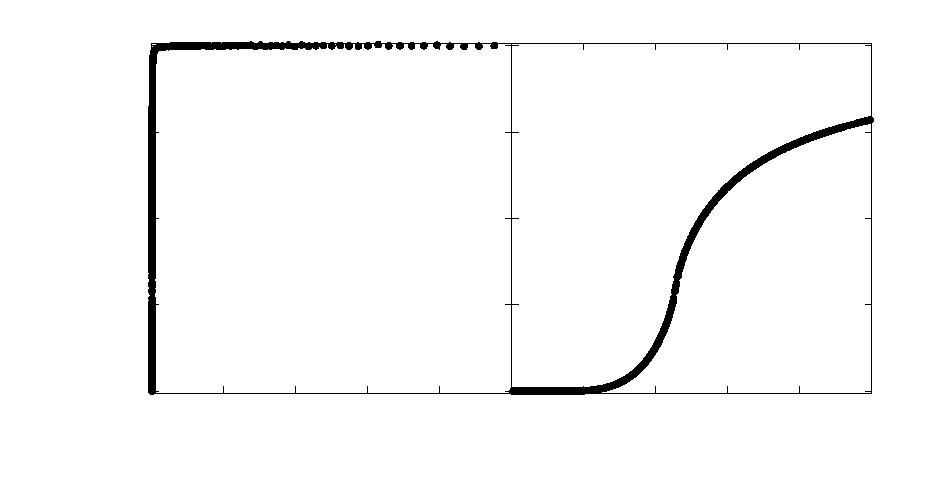
\includegraphics{hamiltonian}}%
    \gplfronttext
  \end{picture}%
\endgroup

		\caption[Hamiltonian in Abhängigkeit von der Temperatur]{Hamiltonian in Abhängigkeit von der Temperatur, gemessen bei Gitterlänge 100, mit Blocklänge 128 zur Fehlerberechnung. Die Fehler sind so klein, dass sie fast nicht sichtbar sind. Dargestellt ist sowohl die Umgebung des kritischen Punktes als auch das asymptotische Verhalten.}
		\label{fig:ergebnishamiltonian}
	\end{figure}
	
%	Dann Akzeptanzrate von wo bis wo, mit gebootstraptem Fehler? Geht auf 1 hoch?
%	\begin{verbatim}
%	test
%	\end{verbatim}

	Die Magnetisierung verhält sich wie nach Gl.~\ref{eq:magnetisierungsgleichungliteratur} erwartet, siehe Abb. \ref{fig:ergebnismagnetisierung}: Bei geringen Temperaturen ist sie eins, danach wird sie kleiner. Bei ca. $T=\num{2,3}$ hat sie einen starken Abfall, und nähert sich danach einem konstanten Wert größer als null an. Nach Gl.~\ref{eq:magnetisierungsgleichungliteratur} wäre zu erwarten, dass der Abfall eine scharfe Kante bildet und danach die Magnetisierung null ist, dies ist allerdings aufgrund der endlichen Gittergröße nicht der Fall, wie in Abschnitt~\ref{sec:isingtheorie} erläutert wird.
	
	%Dia Varianz der Magnetisierung ist sowohl bei niedrigen als auch bei hohen Temperaturen niedrig, ca.{}


	
	\begin{figure}[htbp]
		% GNUPLOT: LaTeX picture with Postscript
\begingroup
  \makeatletter
  \providecommand\color[2][]{%
    \GenericError{(gnuplot) \space\space\space\@spaces}{%
      Package color not loaded in conjunction with
      terminal option `colourtext'%
    }{See the gnuplot documentation for explanation.%
    }{Either use 'blacktext' in gnuplot or load the package
      color.sty in LaTeX.}%
    \renewcommand\color[2][]{}%
  }%
  \providecommand\includegraphics[2][]{%
    \GenericError{(gnuplot) \space\space\space\@spaces}{%
      Package graphicx or graphics not loaded%
    }{See the gnuplot documentation for explanation.%
    }{The gnuplot epslatex terminal needs graphicx.sty or graphics.sty.}%
    \renewcommand\includegraphics[2][]{}%
  }%
  \providecommand\rotatebox[2]{#2}%
  \@ifundefined{ifGPcolor}{%
    \newif\ifGPcolor
    \GPcolortrue
  }{}%
  \@ifundefined{ifGPblacktext}{%
    \newif\ifGPblacktext
    \GPblacktextfalse
  }{}%
  % define a \g@addto@macro without @ in the name:
  \let\gplgaddtomacro\g@addto@macro
  % define empty templates for all commands taking text:
  \gdef\gplbacktext{}%
  \gdef\gplfronttext{}%
  \makeatother
  \ifGPblacktext
    % no textcolor at all
    \def\colorrgb#1{}%
    \def\colorgray#1{}%
  \else
    % gray or color?
    \ifGPcolor
      \def\colorrgb#1{\color[rgb]{#1}}%
      \def\colorgray#1{\color[gray]{#1}}%
      \expandafter\def\csname LTw\endcsname{\color{white}}%
      \expandafter\def\csname LTb\endcsname{\color{black}}%
      \expandafter\def\csname LTa\endcsname{\color{black}}%
      \expandafter\def\csname LT0\endcsname{\color[rgb]{1,0,0}}%
      \expandafter\def\csname LT1\endcsname{\color[rgb]{0,1,0}}%
      \expandafter\def\csname LT2\endcsname{\color[rgb]{0,0,1}}%
      \expandafter\def\csname LT3\endcsname{\color[rgb]{1,0,1}}%
      \expandafter\def\csname LT4\endcsname{\color[rgb]{0,1,1}}%
      \expandafter\def\csname LT5\endcsname{\color[rgb]{1,1,0}}%
      \expandafter\def\csname LT6\endcsname{\color[rgb]{0,0,0}}%
      \expandafter\def\csname LT7\endcsname{\color[rgb]{1,0.3,0}}%
      \expandafter\def\csname LT8\endcsname{\color[rgb]{0.5,0.5,0.5}}%
    \else
      % gray
      \def\colorrgb#1{\color{black}}%
      \def\colorgray#1{\color[gray]{#1}}%
      \expandafter\def\csname LTw\endcsname{\color{white}}%
      \expandafter\def\csname LTb\endcsname{\color{black}}%
      \expandafter\def\csname LTa\endcsname{\color{black}}%
      \expandafter\def\csname LT0\endcsname{\color{black}}%
      \expandafter\def\csname LT1\endcsname{\color{black}}%
      \expandafter\def\csname LT2\endcsname{\color{black}}%
      \expandafter\def\csname LT3\endcsname{\color{black}}%
      \expandafter\def\csname LT4\endcsname{\color{black}}%
      \expandafter\def\csname LT5\endcsname{\color{black}}%
      \expandafter\def\csname LT6\endcsname{\color{black}}%
      \expandafter\def\csname LT7\endcsname{\color{black}}%
      \expandafter\def\csname LT8\endcsname{\color{black}}%
    \fi
  \fi
    \setlength{\unitlength}{0.0500bp}%
    \ifx\gptboxheight\undefined%
      \newlength{\gptboxheight}%
      \newlength{\gptboxwidth}%
      \newsavebox{\gptboxtext}%
    \fi%
    \setlength{\fboxrule}{0.5pt}%
    \setlength{\fboxsep}{1pt}%
\begin{picture}(8640.00,4320.00)%
    \gplgaddtomacro\gplbacktext{%
      \csname LTb\endcsname%
      \put(1164,737){\makebox(0,0)[r]{\strut{}$0$}}%
      \put(1164,1394){\makebox(0,0)[r]{\strut{}$0.2$}}%
      \put(1164,2051){\makebox(0,0)[r]{\strut{}$0.4$}}%
      \put(1164,2708){\makebox(0,0)[r]{\strut{}$0.6$}}%
      \put(1164,3365){\makebox(0,0)[r]{\strut{}$0.8$}}%
      \put(1164,4022){\makebox(0,0)[r]{\strut{}$1$}}%
      \put(1299,484){\makebox(0,0){\strut{}$0$}}%
      \put(1990,484){\makebox(0,0){\strut{}$2000$}}%
      \put(2680,484){\makebox(0,0){\strut{}$4000$}}%
      \put(3370,484){\makebox(0,0){\strut{}$6000$}}%
      \put(4061,484){\makebox(0,0){\strut{}$8000$}}%
      \put(4751,484){\makebox(0,0){\strut{}$10000$}}%
    }%
    \gplgaddtomacro\gplfronttext{%
      \csname LTb\endcsname%
      \put(526,2379){\rotatebox{-270}{\makebox(0,0){\strut{}$M$}}}%
      \put(3023,154){\makebox(0,0){\strut{}Temperatur}}%
    }%
    \gplgaddtomacro\gplbacktext{%
      \csname LTb\endcsname%
      \put(4620,737){\makebox(0,0)[r]{\strut{}}}%
      \put(4620,1394){\makebox(0,0)[r]{\strut{}}}%
      \put(4620,2051){\makebox(0,0)[r]{\strut{}}}%
      \put(4620,2708){\makebox(0,0)[r]{\strut{}}}%
      \put(4620,3365){\makebox(0,0)[r]{\strut{}}}%
      \put(4620,4022){\makebox(0,0)[r]{\strut{}}}%
      \put(4752,484){\makebox(0,0){\strut{}$0$}}%
      \put(5443,484){\makebox(0,0){\strut{}$1$}}%
      \put(6134,484){\makebox(0,0){\strut{}$2$}}%
      \put(6825,484){\makebox(0,0){\strut{}$3$}}%
      \put(7516,484){\makebox(0,0){\strut{}$4$}}%
      \put(8207,484){\makebox(0,0){\strut{}$5$}}%
    }%
    \gplgaddtomacro\gplfronttext{%
      \csname LTb\endcsname%
      \put(6479,154){\makebox(0,0){\strut{}Temperatur}}%
    }%
    \gplbacktext
    \put(0,0){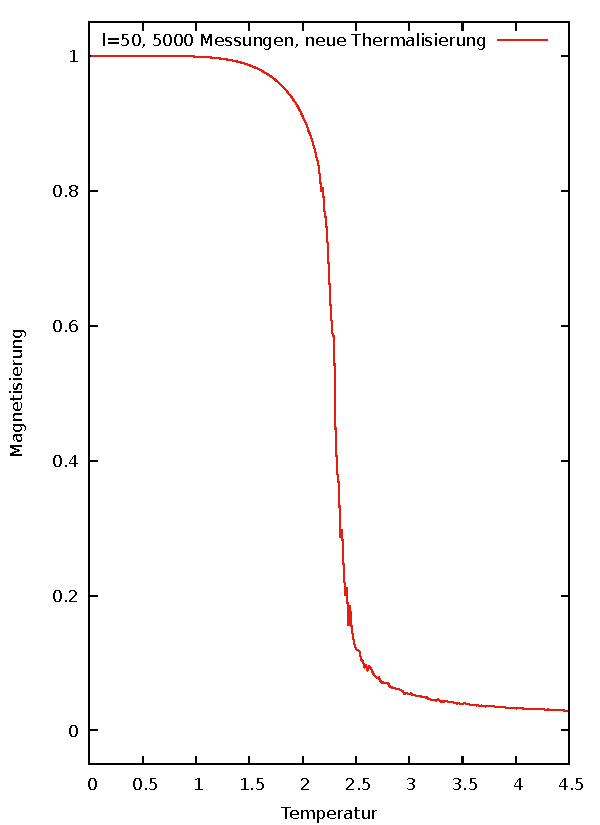
\includegraphics{magnetisierung}}%
    \gplfronttext
  \end{picture}%
\endgroup

		\caption[Magnetisierung in Abhängigkeit von der Temperatur]{Magnetisierung in Abhängigkeit von der Temperatur, gemessen bei Gitterlänge 100, mit Blocklänge 128 zur Fehlerberechnung. Die Fehler sind teilweise so klein, dass sie fast nicht sichtbar sind. Dargestellt ist sowohl die Umgebung des kritischen Punktes als auch das asymptotische Verhalten.}
		\label{fig:ergebnismagnetisierung}
	\end{figure}
	
	In der kritischen Region um $T=\num{2,3}$ herum sind die Standardabweichungen der beobachteten Observablen am größten, außerhalb dieser Region sind sie fast null. Lediglich beim Hamiltonian gibt es bei größeren Temperaturen auch größere Fehler. 
	
	Die Beobachtungen der Observablen zeigen, dass es zwei Phasen gibt: Bei niedrigen Temperaturen sind die Spins im Gitter alle gleich ausgerichtet, das Gitter ändert sich nur sehr wenig pro Messung. Bei hohen Temperaturen sind die Spins im Gitter zufällig ausgerichtet, während einer Messung werden viele Spins umgedreht. Dazwischen findet in der Nähe von $T=\num{2,3}$ ein Phasenübergang statt.
	%Fehler der jeweiligen Messwerte: am größten in Bereich um T=2,2, relativen Fehler angeben? DAvor fast null, danach sehr gering, nur bei Hamiltonian nochmal ein Anstieg bei hohen Temperaturen.
	
	\section{Bestimmung des kritischen Punktes}
	\label{sec:bestkritpunkt}
	
	Der Phasenübergang findet am kritischen Punkt statt. Wie in Abschnitt \ref{sec:isingtheorie} erläutert, ist dort eine Unstetigkeit in der Magnetisierung zu erwarten. Dadurch, dass die Gitterlänge endlich ist, kommt es in der Ableitung der Magnetisierung nach der Temperatur nur zu einem Extremum, nicht zu einer Polstelle. %Zusätzlich kommt es zu einer \enquote{Verschmierung} des kritischen Punktes\cite[vgl. ][S. 104]{binderheermann}.
		
	\begin{figure}[htbp]
		% GNUPLOT: LaTeX picture with Postscript
\begingroup
  \makeatletter
  \providecommand\color[2][]{%
    \GenericError{(gnuplot) \space\space\space\@spaces}{%
      Package color not loaded in conjunction with
      terminal option `colourtext'%
    }{See the gnuplot documentation for explanation.%
    }{Either use 'blacktext' in gnuplot or load the package
      color.sty in LaTeX.}%
    \renewcommand\color[2][]{}%
  }%
  \providecommand\includegraphics[2][]{%
    \GenericError{(gnuplot) \space\space\space\@spaces}{%
      Package graphicx or graphics not loaded%
    }{See the gnuplot documentation for explanation.%
    }{The gnuplot epslatex terminal needs graphicx.sty or graphics.sty.}%
    \renewcommand\includegraphics[2][]{}%
  }%
  \providecommand\rotatebox[2]{#2}%
  \@ifundefined{ifGPcolor}{%
    \newif\ifGPcolor
    \GPcolortrue
  }{}%
  \@ifundefined{ifGPblacktext}{%
    \newif\ifGPblacktext
    \GPblacktextfalse
  }{}%
  % define a \g@addto@macro without @ in the name:
  \let\gplgaddtomacro\g@addto@macro
  % define empty templates for all commands taking text:
  \gdef\gplbacktext{}%
  \gdef\gplfronttext{}%
  \makeatother
  \ifGPblacktext
    % no textcolor at all
    \def\colorrgb#1{}%
    \def\colorgray#1{}%
  \else
    % gray or color?
    \ifGPcolor
      \def\colorrgb#1{\color[rgb]{#1}}%
      \def\colorgray#1{\color[gray]{#1}}%
      \expandafter\def\csname LTw\endcsname{\color{white}}%
      \expandafter\def\csname LTb\endcsname{\color{black}}%
      \expandafter\def\csname LTa\endcsname{\color{black}}%
      \expandafter\def\csname LT0\endcsname{\color[rgb]{1,0,0}}%
      \expandafter\def\csname LT1\endcsname{\color[rgb]{0,1,0}}%
      \expandafter\def\csname LT2\endcsname{\color[rgb]{0,0,1}}%
      \expandafter\def\csname LT3\endcsname{\color[rgb]{1,0,1}}%
      \expandafter\def\csname LT4\endcsname{\color[rgb]{0,1,1}}%
      \expandafter\def\csname LT5\endcsname{\color[rgb]{1,1,0}}%
      \expandafter\def\csname LT6\endcsname{\color[rgb]{0,0,0}}%
      \expandafter\def\csname LT7\endcsname{\color[rgb]{1,0.3,0}}%
      \expandafter\def\csname LT8\endcsname{\color[rgb]{0.5,0.5,0.5}}%
    \else
      % gray
      \def\colorrgb#1{\color{black}}%
      \def\colorgray#1{\color[gray]{#1}}%
      \expandafter\def\csname LTw\endcsname{\color{white}}%
      \expandafter\def\csname LTb\endcsname{\color{black}}%
      \expandafter\def\csname LTa\endcsname{\color{black}}%
      \expandafter\def\csname LT0\endcsname{\color{black}}%
      \expandafter\def\csname LT1\endcsname{\color{black}}%
      \expandafter\def\csname LT2\endcsname{\color{black}}%
      \expandafter\def\csname LT3\endcsname{\color{black}}%
      \expandafter\def\csname LT4\endcsname{\color{black}}%
      \expandafter\def\csname LT5\endcsname{\color{black}}%
      \expandafter\def\csname LT6\endcsname{\color{black}}%
      \expandafter\def\csname LT7\endcsname{\color{black}}%
      \expandafter\def\csname LT8\endcsname{\color{black}}%
    \fi
  \fi
    \setlength{\unitlength}{0.0500bp}%
    \ifx\gptboxheight\undefined%
      \newlength{\gptboxheight}%
      \newlength{\gptboxwidth}%
      \newsavebox{\gptboxtext}%
    \fi%
    \setlength{\fboxrule}{0.5pt}%
    \setlength{\fboxsep}{1pt}%
\begin{picture}(8640.00,6480.00)%
    \gplgaddtomacro\gplbacktext{%
      \csname LTb\endcsname%
      \put(1164,1296){\makebox(0,0)[r]{\strut{}$0$}}%
      \put(1164,2268){\makebox(0,0)[r]{\strut{}$0.2$}}%
      \put(1164,3240){\makebox(0,0)[r]{\strut{}$0.4$}}%
      \put(1164,4211){\makebox(0,0)[r]{\strut{}$0.6$}}%
      \put(1164,5183){\makebox(0,0)[r]{\strut{}$0.8$}}%
      \put(1164,6155){\makebox(0,0)[r]{\strut{}$1$}}%
      \put(1296,1076){\makebox(0,0){\strut{}$1$}}%
      \put(2448,1076){\makebox(0,0){\strut{}$1.5$}}%
      \put(3600,1076){\makebox(0,0){\strut{}$2$}}%
      \put(4752,1076){\makebox(0,0){\strut{}$2.5$}}%
      \put(5903,1076){\makebox(0,0){\strut{}$3$}}%
      \put(7055,1076){\makebox(0,0){\strut{}$3.5$}}%
      \put(8207,1076){\makebox(0,0){\strut{}$4$}}%
    }%
    \gplgaddtomacro\gplfronttext{%
      \csname LTb\endcsname%
      \put(526,3725){\rotatebox{-270}{\makebox(0,0){\strut{}$M$}}}%
      \put(4751,746){\makebox(0,0){\strut{}Temperatur}}%
      \csname LTb\endcsname%
      \put(7220,5982){\makebox(0,0)[r]{\strut{}$\text{laenge}=120$}}%
      \csname LTb\endcsname%
      \put(7220,5762){\makebox(0,0)[r]{\strut{}$\text{laenge}=36$}}%
      \csname LTb\endcsname%
      \put(7220,5542){\makebox(0,0)[r]{\strut{}Theorie}}%
    }%
    \gplbacktext
    \put(0,0){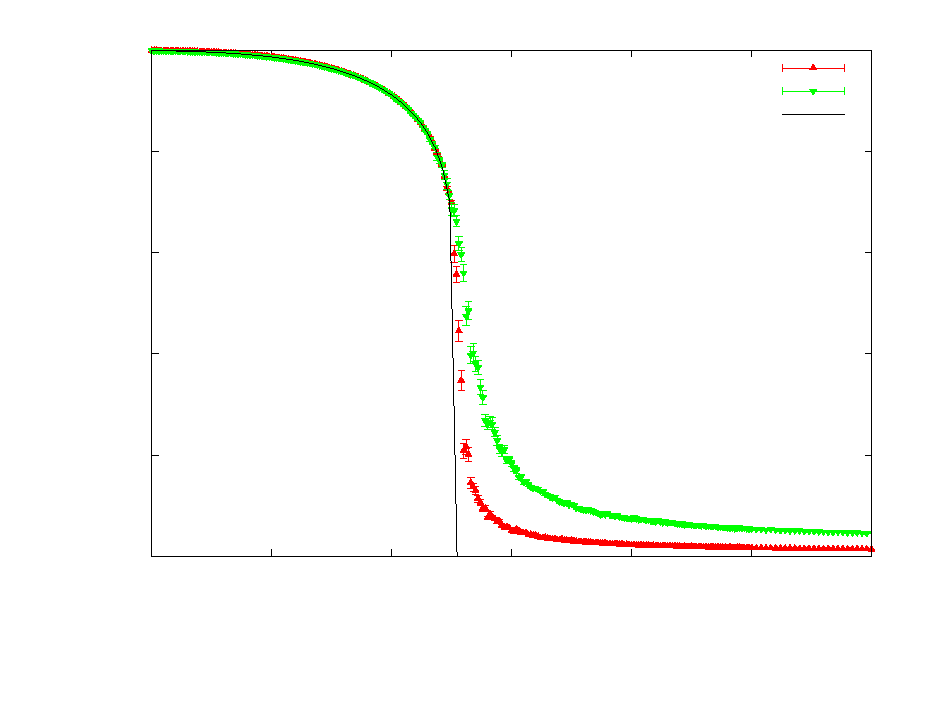
\includegraphics{magnetisierunglaenge}}%
    \gplfronttext
  \end{picture}%
\endgroup

		\caption[Magnetisierung bei verschiedenen Gitterlängen und Verwendung von OpenMP]{Magnetisierung bei verschiedenen Gitterlängen, verglichen mit Literaturergebnis, Werte bestimmt mit Blocklänge 128 zur Fehlerberechnung, parallelisiert mit OpenMP.}
		\label{fig:maglaenge}
	\end{figure}

	
	Für $J=1$ wird der kritische Punkt nach Gl. \ref{eq:kritischetemperatur} bei $T=\num{2,269}$ erwartet.
	Um zu sehen, wie gut die Monte-Carlo-Simulation die analytisch bestimmte Erwartung reproduziert, wurde die Magnetisierung für verschiedene Gitterlängen bestimmt, mit besonders vielen Messpunkten in der Region, in der der kritische Punkt erwartet wird. Beim Vergleich der Ergebnisse in Abb.~\ref{fig:maglaenge} fällt auf, dass der Abfall der Magnetisierung bei größeren Gitterlängen steiler ist. Der Wert, den die Magnetisierung oberhalb der kritischen Temperatur annimmt, ist geringer für größere Gitterlängen. Dieses Verhalten entspricht den Erwartungen für endliche Gitterlängen aus Abschnitt~\ref{sec:isingtheorie}. Bei Parallelisierung mit MPI, dargestellt in Abb.~\ref{fig:maglaengempi}, verhalten sich die Ergebnisse genauso wie bei Parallelisierung mit OpenMP~\ref{fig:maglaenge}.
	
	
	\begin{figure}[htbp]
		\input{Bilder/magnetisierunglaengempi}
		\caption[Magnetisierung bei verschiedenen Gitterlängen und Verwendung von MPI]{Magnetisierung bei verschiedenen Gitterlängen, verglichen mit Literaturergebnis, Werte bestimmt mit Blocklänge 128 zur Fehlerberechnung, parallelisiert mit MPI.}
		\label{fig:maglaengempi}
	\end{figure}

	Für verschiedene Gitterlängen wird die kritische Temperatur bestimmt. Diese ist die Stelle, wo die Ableitung am kleinsten ist, die Kurve der Magnetisierung also am steilsten verläuft. Die so bestimmten Werte der kritischen Temperatur sind in Abb. \ref{fig:tkritlaenge} zu sehen. Die meisten Werte sind größer, als von der Theorie vorhergesagt, die größte Abweichung nach oben beträgt 6\%. Einige Werte sind auch kleiner, die größte Abweichung nach unten beträgt $\num{1,1}\%$. Auch bei gleichen Gitterlängen sind die mit MPI und mit OpenMP bestimmten Werte unterschiedlich, dies liegt daran, dass bei den unterschiedlichen Methoden unterschiedliche Zufallszahlen zum Einsatz kommen und sich somit die Ergebnisse leicht unterscheiden. Bei beiden ist das Verhalten jedoch gleich: Bei kleinen Gitterlängen sind die Werte stark um den theoretisch erwarteten Wert gestreut, diese Streuung nimmt jedoch mit zunehmender Gitterlänge ab. Die kritische Temperatur nähert sich asymptotisch dem erwarteten Ergebnis an.
	%Alle Schätzer sind größer als die theoretische erwartete Temperatur, jedoch beträgt die größte Abweichung nur ca 6\%. Die Schätzer variieren stark, jedoch sind sie bei kleineren Gitterlängen eher größer und scheinen sich asymptotisch dem theoretisch erwarteten Wert anzunähern.
	
	\begin{figure}[htbp]
		\input{Bilder/tkritvonl}
		\caption[kritische Temperatur in Abhängigkeit von der Gitterlänge]{kritische Temperatur in Abhängigkeit von der Gitterlänge. Untersucht wurde die Ableitung der Werte, die mit Blocklänge 128 bestimmt wurden}
		\label{fig:tkritlaenge}
	\end{figure}

	%Schätzer für kritische Temperatur: Temperatur bei der die Ableitung Minimum hat. Für verschiedene Gitterlängen bestimmt, siehe Abb. \ref{fig:tkritlaenge}. Schon bei geringen Gitterlängen wie 12 Abweichungne nicht größer als 6\% vom erwarteten Wert. bestimmte tkrit variiert zwischen Gitterlängen, ist aber immer größer als erwarteter Wert. Variation scheint abzunehmen und Tkrit scheint sich asymptotisch dem erwarteten Wert anzunähern.
	
	%\newpage

	Die Monte-Carlo-Simulationen reproduzieren also gut die Ergebnisse der analytischen Betrachtung aus Abschnitt~\ref{sec:isingtheorie}. Je größer die Gitterlänge ist, desto ähnlicher sind die Simulationsergebnisse zu der Theorie. Aufgrund der Parallelisierung der Messungen konnte dies auch insbesondere für große Gitterlängen bestätigt werden. Dabei hat sich gezeigt, dass beide möglichen Arten der Parallelisierung, \textit{shared} und \textit{distributed memory}, zum gleichen Ergebnis führen.
	%Zeigt, dass Simulation gut analytische Werte reproduziert.
	
	%Abschlusssatz?
	%Die jeweilige Schätzung für den kritischen Punkt wurde bestimmt Ableitung Zwei/Dreipunkt, Magnetisierung oder sqrt(mag*mag)? Alles in der Region des erwarteten kritischen Punktes, eventuell für größere Gitterlängen näher?
	
%	
%		\begin{figure}[htbp]
%			\input{Bilder/akzeptanzratefehler}
%			\caption{Fehler Akzeptanzrate}
%			\label{fig:fehlersakzeptanzrate}
%		\end{figure}
%		\begin{figure}[htbp]
%			\input{Bilder/magnetisierungfehler}
%			\caption{Fehler Magnetisierung}
%			\label{fig:fehlermagnetisierung}
%		\end{figure}
%		\begin{figure}[htbp]
%			\input{Bilder/hamiltonianfehler}
%			\caption{Fehler Hamiltonian}
%			\label{fig:fehlerhamiltonian}
%		\end{figure}
	%Mittels der Zwei-Punkt-Formel wurde zusätzlich die Ableitung der Magnetisierung bestimmt, und damit der Schätzer für die kritische Temperatur in Abhängigkeit der Gitterlänge bestimmt. Als Fehler der Abschätzung wurde jeweils der Abstand zum nächsten Punkt angenommen. Wie man an Bild \ref{fig:tkritlaenge} sieht, nähert sich die kritische Temperatur mit steigender Gitterlänge asymptotisch an den erwarteten Wert an. 
	
	
	%Wie bei der Diskussion von	
	
	%Dann Magnetisierung: Vergleich zweier Längen, Erklärung finite size Effekts wie in Binder-Heermann erwähnt.
%	In Bild~\ref{fig:ergebnismagnetisierung} ist dieses Verhalten zu sehen. In Bild~\ref{fig:maglaenge} ist dies noch deutlicher zu sehen, dort wird die Magnetisierung bei zwei verschiedenen Gitterlängen miteinander verglichen. Es fällt auf, dass bei kleineren Längen der Abfall der Magnetisierung weniger steil ist, sowie die Magnetisierung oberhalb des kritischen Punktes einen größeren Wert hat. Auch dies deckt sich mit den Erwartungen aus~\cite[S. 45 f.]{binderheermann}.%, ebenso wie der Vergleich zweier Längen: bei kleineren Gitterlängen ist der Abfall weniger steil und der Wert der Magnetisierung bei hohen Temperaturen größer.
%	
%	
%	\begin{figure}[htbp]
%		% GNUPLOT: LaTeX picture with Postscript
\begingroup
  \makeatletter
  \providecommand\color[2][]{%
    \GenericError{(gnuplot) \space\space\space\@spaces}{%
      Package color not loaded in conjunction with
      terminal option `colourtext'%
    }{See the gnuplot documentation for explanation.%
    }{Either use 'blacktext' in gnuplot or load the package
      color.sty in LaTeX.}%
    \renewcommand\color[2][]{}%
  }%
  \providecommand\includegraphics[2][]{%
    \GenericError{(gnuplot) \space\space\space\@spaces}{%
      Package graphicx or graphics not loaded%
    }{See the gnuplot documentation for explanation.%
    }{The gnuplot epslatex terminal needs graphicx.sty or graphics.sty.}%
    \renewcommand\includegraphics[2][]{}%
  }%
  \providecommand\rotatebox[2]{#2}%
  \@ifundefined{ifGPcolor}{%
    \newif\ifGPcolor
    \GPcolortrue
  }{}%
  \@ifundefined{ifGPblacktext}{%
    \newif\ifGPblacktext
    \GPblacktextfalse
  }{}%
  % define a \g@addto@macro without @ in the name:
  \let\gplgaddtomacro\g@addto@macro
  % define empty templates for all commands taking text:
  \gdef\gplbacktext{}%
  \gdef\gplfronttext{}%
  \makeatother
  \ifGPblacktext
    % no textcolor at all
    \def\colorrgb#1{}%
    \def\colorgray#1{}%
  \else
    % gray or color?
    \ifGPcolor
      \def\colorrgb#1{\color[rgb]{#1}}%
      \def\colorgray#1{\color[gray]{#1}}%
      \expandafter\def\csname LTw\endcsname{\color{white}}%
      \expandafter\def\csname LTb\endcsname{\color{black}}%
      \expandafter\def\csname LTa\endcsname{\color{black}}%
      \expandafter\def\csname LT0\endcsname{\color[rgb]{1,0,0}}%
      \expandafter\def\csname LT1\endcsname{\color[rgb]{0,1,0}}%
      \expandafter\def\csname LT2\endcsname{\color[rgb]{0,0,1}}%
      \expandafter\def\csname LT3\endcsname{\color[rgb]{1,0,1}}%
      \expandafter\def\csname LT4\endcsname{\color[rgb]{0,1,1}}%
      \expandafter\def\csname LT5\endcsname{\color[rgb]{1,1,0}}%
      \expandafter\def\csname LT6\endcsname{\color[rgb]{0,0,0}}%
      \expandafter\def\csname LT7\endcsname{\color[rgb]{1,0.3,0}}%
      \expandafter\def\csname LT8\endcsname{\color[rgb]{0.5,0.5,0.5}}%
    \else
      % gray
      \def\colorrgb#1{\color{black}}%
      \def\colorgray#1{\color[gray]{#1}}%
      \expandafter\def\csname LTw\endcsname{\color{white}}%
      \expandafter\def\csname LTb\endcsname{\color{black}}%
      \expandafter\def\csname LTa\endcsname{\color{black}}%
      \expandafter\def\csname LT0\endcsname{\color{black}}%
      \expandafter\def\csname LT1\endcsname{\color{black}}%
      \expandafter\def\csname LT2\endcsname{\color{black}}%
      \expandafter\def\csname LT3\endcsname{\color{black}}%
      \expandafter\def\csname LT4\endcsname{\color{black}}%
      \expandafter\def\csname LT5\endcsname{\color{black}}%
      \expandafter\def\csname LT6\endcsname{\color{black}}%
      \expandafter\def\csname LT7\endcsname{\color{black}}%
      \expandafter\def\csname LT8\endcsname{\color{black}}%
    \fi
  \fi
    \setlength{\unitlength}{0.0500bp}%
    \ifx\gptboxheight\undefined%
      \newlength{\gptboxheight}%
      \newlength{\gptboxwidth}%
      \newsavebox{\gptboxtext}%
    \fi%
    \setlength{\fboxrule}{0.5pt}%
    \setlength{\fboxsep}{1pt}%
\begin{picture}(8640.00,6480.00)%
    \gplgaddtomacro\gplbacktext{%
      \csname LTb\endcsname%
      \put(1164,1296){\makebox(0,0)[r]{\strut{}$0$}}%
      \put(1164,2268){\makebox(0,0)[r]{\strut{}$0.2$}}%
      \put(1164,3240){\makebox(0,0)[r]{\strut{}$0.4$}}%
      \put(1164,4211){\makebox(0,0)[r]{\strut{}$0.6$}}%
      \put(1164,5183){\makebox(0,0)[r]{\strut{}$0.8$}}%
      \put(1164,6155){\makebox(0,0)[r]{\strut{}$1$}}%
      \put(1296,1076){\makebox(0,0){\strut{}$1$}}%
      \put(2448,1076){\makebox(0,0){\strut{}$1.5$}}%
      \put(3600,1076){\makebox(0,0){\strut{}$2$}}%
      \put(4752,1076){\makebox(0,0){\strut{}$2.5$}}%
      \put(5903,1076){\makebox(0,0){\strut{}$3$}}%
      \put(7055,1076){\makebox(0,0){\strut{}$3.5$}}%
      \put(8207,1076){\makebox(0,0){\strut{}$4$}}%
    }%
    \gplgaddtomacro\gplfronttext{%
      \csname LTb\endcsname%
      \put(526,3725){\rotatebox{-270}{\makebox(0,0){\strut{}$M$}}}%
      \put(4751,746){\makebox(0,0){\strut{}Temperatur}}%
      \csname LTb\endcsname%
      \put(7220,5982){\makebox(0,0)[r]{\strut{}$\text{laenge}=120$}}%
      \csname LTb\endcsname%
      \put(7220,5762){\makebox(0,0)[r]{\strut{}$\text{laenge}=36$}}%
      \csname LTb\endcsname%
      \put(7220,5542){\makebox(0,0)[r]{\strut{}Theorie}}%
    }%
    \gplbacktext
    \put(0,0){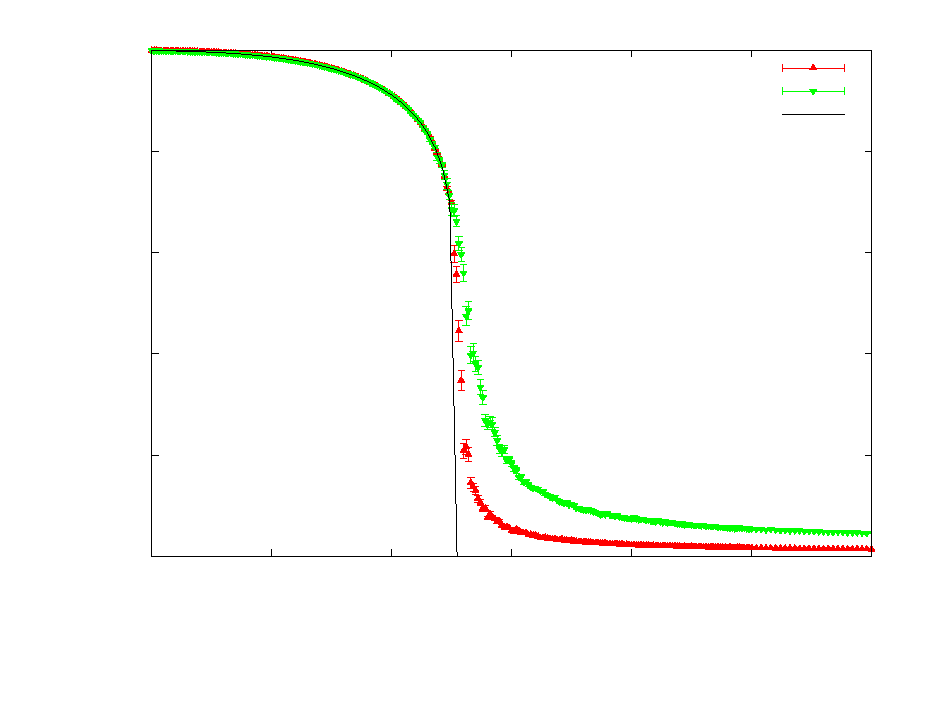
\includegraphics{magnetisierunglaenge}}%
    \gplfronttext
  \end{picture}%
\endgroup

%		\caption[Magnetisierung bei verschiedenen Längen]{Magnetisierung bei verschiedenen Längen, Fehler gemessen mit Blocklänge 128}
%		\label{fig:maglaenge}
%	\end{figure}
%
%	\begin{figure}[htbp]
%		% GNUPLOT: LaTeX picture with Postscript
\begingroup
  \makeatletter
  \providecommand\color[2][]{%
    \GenericError{(gnuplot) \space\space\space\@spaces}{%
      Package color not loaded in conjunction with
      terminal option `colourtext'%
    }{See the gnuplot documentation for explanation.%
    }{Either use 'blacktext' in gnuplot or load the package
      color.sty in LaTeX.}%
    \renewcommand\color[2][]{}%
  }%
  \providecommand\includegraphics[2][]{%
    \GenericError{(gnuplot) \space\space\space\@spaces}{%
      Package graphicx or graphics not loaded%
    }{See the gnuplot documentation for explanation.%
    }{The gnuplot epslatex terminal needs graphicx.sty or graphics.sty.}%
    \renewcommand\includegraphics[2][]{}%
  }%
  \providecommand\rotatebox[2]{#2}%
  \@ifundefined{ifGPcolor}{%
    \newif\ifGPcolor
    \GPcolortrue
  }{}%
  \@ifundefined{ifGPblacktext}{%
    \newif\ifGPblacktext
    \GPblacktextfalse
  }{}%
  % define a \g@addto@macro without @ in the name:
  \let\gplgaddtomacro\g@addto@macro
  % define empty templates for all commands taking text:
  \gdef\gplbacktext{}%
  \gdef\gplfronttext{}%
  \makeatother
  \ifGPblacktext
    % no textcolor at all
    \def\colorrgb#1{}%
    \def\colorgray#1{}%
  \else
    % gray or color?
    \ifGPcolor
      \def\colorrgb#1{\color[rgb]{#1}}%
      \def\colorgray#1{\color[gray]{#1}}%
      \expandafter\def\csname LTw\endcsname{\color{white}}%
      \expandafter\def\csname LTb\endcsname{\color{black}}%
      \expandafter\def\csname LTa\endcsname{\color{black}}%
      \expandafter\def\csname LT0\endcsname{\color[rgb]{1,0,0}}%
      \expandafter\def\csname LT1\endcsname{\color[rgb]{0,1,0}}%
      \expandafter\def\csname LT2\endcsname{\color[rgb]{0,0,1}}%
      \expandafter\def\csname LT3\endcsname{\color[rgb]{1,0,1}}%
      \expandafter\def\csname LT4\endcsname{\color[rgb]{0,1,1}}%
      \expandafter\def\csname LT5\endcsname{\color[rgb]{1,1,0}}%
      \expandafter\def\csname LT6\endcsname{\color[rgb]{0,0,0}}%
      \expandafter\def\csname LT7\endcsname{\color[rgb]{1,0.3,0}}%
      \expandafter\def\csname LT8\endcsname{\color[rgb]{0.5,0.5,0.5}}%
    \else
      % gray
      \def\colorrgb#1{\color{black}}%
      \def\colorgray#1{\color[gray]{#1}}%
      \expandafter\def\csname LTw\endcsname{\color{white}}%
      \expandafter\def\csname LTb\endcsname{\color{black}}%
      \expandafter\def\csname LTa\endcsname{\color{black}}%
      \expandafter\def\csname LT0\endcsname{\color{black}}%
      \expandafter\def\csname LT1\endcsname{\color{black}}%
      \expandafter\def\csname LT2\endcsname{\color{black}}%
      \expandafter\def\csname LT3\endcsname{\color{black}}%
      \expandafter\def\csname LT4\endcsname{\color{black}}%
      \expandafter\def\csname LT5\endcsname{\color{black}}%
      \expandafter\def\csname LT6\endcsname{\color{black}}%
      \expandafter\def\csname LT7\endcsname{\color{black}}%
      \expandafter\def\csname LT8\endcsname{\color{black}}%
    \fi
  \fi
    \setlength{\unitlength}{0.0500bp}%
    \ifx\gptboxheight\undefined%
      \newlength{\gptboxheight}%
      \newlength{\gptboxwidth}%
      \newsavebox{\gptboxtext}%
    \fi%
    \setlength{\fboxrule}{0.5pt}%
    \setlength{\fboxsep}{1pt}%
\begin{picture}(8640.00,6480.00)%
    \gplgaddtomacro\gplbacktext{%
      \csname LTb\endcsname%
      \put(1164,1296){\makebox(0,0)[r]{\strut{}$-18$}}%
      \put(1164,1738){\makebox(0,0)[r]{\strut{}$-16$}}%
      \put(1164,2179){\makebox(0,0)[r]{\strut{}$-14$}}%
      \put(1164,2621){\makebox(0,0)[r]{\strut{}$-12$}}%
      \put(1164,3063){\makebox(0,0)[r]{\strut{}$-10$}}%
      \put(1164,3505){\makebox(0,0)[r]{\strut{}$-8$}}%
      \put(1164,3946){\makebox(0,0)[r]{\strut{}$-6$}}%
      \put(1164,4388){\makebox(0,0)[r]{\strut{}$-4$}}%
      \put(1164,4830){\makebox(0,0)[r]{\strut{}$-2$}}%
      \put(1164,5272){\makebox(0,0)[r]{\strut{}$0$}}%
      \put(1164,5713){\makebox(0,0)[r]{\strut{}$2$}}%
      \put(1164,6155){\makebox(0,0)[r]{\strut{}$4$}}%
      \put(1296,1076){\makebox(0,0){\strut{}$1$}}%
      \put(2448,1076){\makebox(0,0){\strut{}$1.5$}}%
      \put(3600,1076){\makebox(0,0){\strut{}$2$}}%
      \put(4752,1076){\makebox(0,0){\strut{}$2.5$}}%
      \put(5903,1076){\makebox(0,0){\strut{}$3$}}%
      \put(7055,1076){\makebox(0,0){\strut{}$3.5$}}%
      \put(8207,1076){\makebox(0,0){\strut{}$4$}}%
    }%
    \gplgaddtomacro\gplfronttext{%
      \csname LTb\endcsname%
      \put(526,3725){\rotatebox{-270}{\makebox(0,0){\strut{}$\dpd{M}{T}$}}}%
      \put(4751,746){\makebox(0,0){\strut{}Temperatur}}%
    }%
    \gplbacktext
    \put(0,0){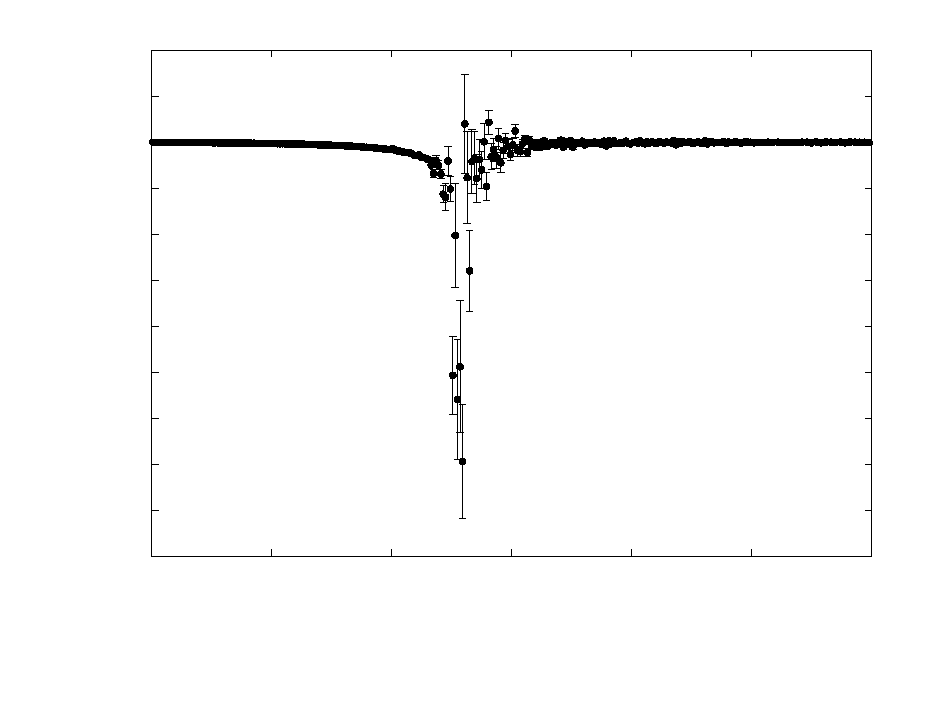
\includegraphics{ableitung120128}}%
    \gplfronttext
  \end{picture}%
\endgroup

%		\caption[Ableitung der Magnetisierung]{Ableitung der Magnetisierung, berechnet mit Zwei-Punkt-Formel. Fehler mit Gaußscher Fehlerfortpflanzung aus den Fehlern bei Blocklänge 128 bestimmt}
%		\label{fig:ableitung120128}
%	\end{figure}
%	
%	In Bild~\ref{fig:maglaenge} ist zusätzlich die nach Gl.~\ref{eq:magnetisierungsgleichungliteratur} erwartete Magnetisierung eingezeichnet. Bis zum theoretischen kritischen Punkt, nach Gl.~\ref{eq:kritischetemperatur} bei $T=\num{2,269}$, liegen alle Messdaten in ihren Fehlergrenzen auf der erwarteten Kurve, erst danach kommt es aufgrund des weniger starken Abfalls zu Abweichungen.
%	
%	Um den kritischen Punkt genauer zu bestimmen, wird zusätzlich mit der Zwei-Punkt-Formel die Ableitung der gemessenen Magnetisierung bestimmt, siehe Bild~\ref{fig:ableitung120128}. Dort wird sichtbar, dass die Änderungsrate der Magnetisierung meist sehr klein ist, nur um den kritischen Punkt herum ist sie groß.% Die größte Änderung fand im Intervall $2,285\pm0,1$ statt, dies ist minimal größer als der theoretisch erwartete kritische Punkt, die Abweichung beträgt $1,5 \sigma$. 
%	Vergleich gemessene/theoretische Magnetisierung: Nur graphisch oder auch Rechnerisch: Anpassung an Bereich mit Fehlern != 0?
	%Größte Ableitung bei 2,285 pm 0,1 bei Länge 120.
	
	%Bestimmung kritischer Punkt? Über ableitung? Oder Kumulante wie in Binder/Herrmann?
	%Theoretischer Kritischer Punkt: J*2,269
%	Messungen mit QBiG, bei denen nur die Zeit zum Durchführen von 1000 Messungen bei verschiedenen Längen und mit verschieden vielen benutzten Kernen gemessen wurde, zeigen, dass bei kleinen Längen wie 10 die benötigte Zeit mit Anzahl der Kerne sogar zunimmt. Dies ist auf den Overhead zurückzuführen.
%		
%	
%	Messungen auf Intel(R) Core(TM) i7-7500U CPU @ 2.70GHz, lcpunode01 und lcpunode02 auf QBiG.